\chapter{Avaliação}
\label{cap:avaliacao}

%Durante as fases de análise e desenvolvimento existiu sempre a preocupação de efectuar uma análise funcional e de desempenho.



%\section{Ferramenta de testes e}
%Como efectuar a monitorização

%Foi desenvolvida uma aplicação para testar o desenvolvimento da ferramenta.
%Esta aplicação 

%\subsection{Test Unit}

%De forma a testar o repositório de dados foram efectuados diferentes \textit{unit tests}, de forma a assegurar que todas as alterações efectuadas na ferramenta ficavam de correctas.

%\subsection{Aplicação Monitora}
%\label{sub:monitor_app}

%Para poder mais facilmente efectuar os testes de avaliação, foi criado uma ferramenta em nível utilizador que permite lançar a aplicação e configurar automaticamente o sistema para a monitorizar. Esta verifica o identificador do processos e o momento em que se dá o inicio e o fim da sua execução, de forma a iniciar e terminar a monitorização quando necessário.

%\subsection{Aplicação de testes de performance}

%Para ajudar na avaliação da ferramenta desenvolvida foi criado um conjunto de aplicações independentes ( scripts e aplicações ) para monitorizar a actividade de algumas aplicações que se consideraram pertinentes no processo de avaliação do desempenho da ferramenta.

%A aplicação desenvolvida \textit{manager} tem de ser executada sob o controlo do utilizador \textit{root}, devido à necessidade de executar processos que só este utilizador tem acesso. Estes processos anteriormente mencionados são \textit{insmod}, \textit{rmmod} e \textit{tcpdump}.

%Os \textit{scripts} \textit{bash} criados serviram para obter o número de dados e pacotes transferidos na interface, bem como fazer a separação dos tempos que as aplicações de testes executaram para conseguir automatizar o processo de execução e recolha de dados dos testes.


%\section{Temporizadores}

%Temporizadores no núcleo do sistema.


%\subsection{Temporizadores de Alta-Resolução}

%\textit{HrTimer}


%----------------------------------------------------------------------------------------------------------

Antes de se utilizar um novo sistema, é conveniente proceder-se a testes alargados de verificação, para que se tome conhecimento do seu correcto funcionamento e das sobrecargas introduzidas, que de modo a este possa ser utilizado como uma mais–valia. 
O mecanismo implementado (\textit{MRoP}) foi avaliado funcionalmente através da utilização de programas específicos para a transferência de dados, baseados nos protocolos \textit{ftp}, \textit{http} e na aplicação de análise de desempenho e largura de banda \textit{iperf}.
Para esse efeito recorreu-se a um conjunto alargado de testes, tendo como principal objectivo verificar o correcto funcionamento da aplicação, a capacidade de capturar todos os pacotes envolvidos nas comunicações do processo alvo (e apenas estes), bem como o seu desempenho e a sobrecarga introduzida.
A verificação da captura dos pacotes envolvidos nas comunicações do processo alvo foi realizada, recorrendo à ferramenta \textit{WireShark} (processo esse, descrito na secção \ref{sec:eval_functional}).
Tendo em vista a realização de testes que avaliam o desempenho da aplicação, foram utilizadas duas máquinas, conectadas directamente, conforme o descrito  na secção \ref{sec:eval_performance}.
Por fim abordar-se-à, detalhadamente, o desempenho efectivo da aplicação.


\section{Avaliação Funcional}
\label{sec:eval_functional}


A análise funcional foi efectuada recorrendo a programas simples, que desencadeavam chamadas sucessivas de criação, comunicação e remoção de \textit{sockets}, verificando-se o estado dos mesmos (relativamente aos portos e endereços), nos \textit{handlers} das funções instrumentadas no núcleo.
Como os dados relativos aos \textit{sockets} ficavam no repositório de dados, foi possível obter também aqui a verificação, através do ficheiro criado no \textit{DebugFs}, que os dados estavam correctos e de acordo com o que a função de filtragem iria utilizar.

No \textit{handler} os dados obtidos oriundos são os oriundos da applicação, ou seja ainda sujeitos a verificação pelo núcleo.
A funções instrumentadas foram \textit{sys\_connect}, \textit{sys\_accept}, \textit{sys\_bind}, \textit{sys\_recvfrom}, \textit{sys\_sendto} e \textit{close ...}, através da instrumentação destas funções foi possível obter todas as interacções com o exterior via rede, realizadas pelas aplicações.


O ficheiro responsável destes dados, contém toda a informação relativa aos portos e endereços em utilização, por parte da aplicação monitorizada.
Deste modo, efectua a comparação dos dados produzidos e valida esta análise utilizando, para além de comportar com o próprio programa, foi a ferramenta (\textit{netstat}), que indicou os portos e endereços utilizados pelos processos no sistema.
A ferramenta anteriormente referida, utiliza o sistema de ficheiros virtual \textit{ProcFs}, para obter os dados relativos aos portos e endereços utilizados,  de modo a estabelecer uma análise comparativa com os dados produzidos pelo \textit{MRoP}.

Para além desta verificação, foi efectuada a confirmação de que todos os pacotes pertencentes às comunicações foram, de facto, correctamente capturadas.
Para tal, recorreu-se à captura de pacotes, por intermédio do \textit{TcpDump} com o módulo \textit{MRoP} activo.
Através deste procedimento constatou-se que todo o tráfego, referente aos protocolos (\textit{ftp} e \textit{http}), estava de facto completo e correcto, desde a abertura ao fecho das conexões, não existindo pacotes pertencentes a outros processos na captura.
Esta validação foi ainda conseguida, por intermédio da utilização do programa \textit{WireShark}, o qual permitiu identificar os fluxos de dados referentes aos protocolos das novas aplicações alvo.


Foram criados dois sistema simples de cliente/servidor, um utilizando canais \textit{tcp} e o canais \textit{udp}, de modo a verificar como ambos os protocolos apresentam as suas informações no núcleo.
Os servidores esperavam conecções numa porta escolhida previamente, permitindo que os clientes efectuassem conecções para estes.
Nos servidores e nos clientes eram apresentados os endereços de memória da estrutura de dados (\textit{struct sockaddr}), que contém as propriedades dos \textit{sockets}, tais como, porto, endereço, protocolo, etc.

A utilização de \textit{KRetProbes} permitiu que se garantisse a correcção dos dados, uma vez que se os dados não estivessem de acordo com o esperado, o núcleo através do valor de retorno indicaria que existia algum problema.
Estas situações estão contempladas dado que na função de \textit{handler} de retorno, um dos primeiros dados a verificar é o valor de retorno indicado pela função instrumentada, caso este valor seja de erro, todas as alterações previamente introduzidas no repositório serão removidas, deixando assim o repositório consistente com o núcleo.

Após a monitorização de rede, foi possível recuperar o ficheiro que foi transmitido via rede utilizando o \textit{Wireshark}

Foram também efectuados testes para verificar que apesar de um processos estar em execução, quando se indicava ao \textit{MRoP} qual o processo a monitorizar, este analisava todos os canais pertencentes ao processo, procedendo em seguida à inserção dos portos, endereços e protocolos, no repositório.
Terminado esta primeira análise eram verificados se todos os canais de rede, relativamente aos protocolos \textit{tcp} e \textit{udp} estavam com as informações correctas e em igual número ao que era reportado através do programa \textit{netstat}, respectivamente ao processo.


\section{Avaliação do desempenho}
\label{sec:eval_performance}

Tendo presente a avaliação do desempenho, foram efectuados diversos testes com o objectivo de avaliar a sobrecarga gerada pela introdução do \textit{MRoP}.
Estes testes basearam-se na recepção ou transmissão de \textit{1 GigaByte} de dados, utilizando diferentes programas e protocolos.
Ambas as máquinas, que se optou por designar de máquina 1 e máquina 2, procederam à transmissão/recepção de dados, utilizando cada uma, apenas, um processador activo de 2 e de 2.6 Ghz, respectivamente.
As máquinas anteriormente descritas encontravam-se conectadas directamente, por interfaces de rede a 100 MBit/s, ficando uma das máquinas responsável pela execução dos servidores \textit{ftp}, \textit{http} e \textit{iperf}, e a outra pelos respectivos clientes.
A versão do sistema de operação utilizado, em ambas as máquinas, correspondeu ao 2.6.39, sendo que na máquina 1 foram introduzidas as modificações, para incluir o \textit{hook} do \textit{MRoP} e as suas funções auxiliares, enquanto na máquina 2 se executou o sistema original.

\subsection{Desempenho do MRoP}


Na execução destes testes, foram efectuadas dez iterações, isto é, cada teste foi executado dez vezes, para cada experiência considerada, de modo a obter um valor médio e um desvio padrão considerado aceitável.
os testes efectuados, em particular os primeiros, ilustram situações em que não há grande vantagem em ter o sistema o \textit{MRoP} activo, com vista a medir a sobrecarga do \textit{MRoP}.
Os resultados obtidos constam nas tabelas \ref{tab:desempenho} e \ref{tab:overhead}:

\begin{table}[!htb]
\begin{center}
\caption{Tempos médios em segundos (s)}
\begin{tabular}{ | c | c | c | c |  }
\hline
Teste & \hspace {0.3cm} Original \hspace {0.3cm}& \hspace {0.2cm} Com TcpDump \hspace {0.2cm} & Com TcpDump e MRoP \\
\hline
1GB - FTP$^{1}$ & 91.8508	& 91.8500 & 91.8854 \\
1GB - HTTP$^{2}$ & 91.6391 & 91.6472 & 91.6674 \\ 
IPerf - 1GB TCP$^{3}$ & 91.3790	& 91.2535	& 91.2672 \\
IPerf - 1GB UDP$^{4}$ & 89.7975 & 89.8007 & 89.8464 \\
\hline
\hline
1GB HTTP - 2 conexões$^{5}$ & 182.1573 & 188.7156 & 182.0161 \\
IPerf - 1GB UDP 2 conexões$^{6}$ & 179.4930 & 179.6280 & 179.6369 \\
\hline
\end{tabular}
\label{tab:desempenho}
\end{center}
\end{table}

\begin{table}[!htb]
\begin{center}
\caption{Sobrecarga das transferências (valores em percentagem)}
\begin{tabular}{ | c | c | c |}
\hline
Teste & \hspace {0.3cm} TcpDump \hspace {0.3cm} & TcpDump com MRoP  \\

\hline
1GB - FTP$^{1}$ & -0.0009  & 0.0377  \\
1GB - HTTP$^{2}$ & 0.0088 &  0.0309   \\
IPerf - 1GB TCP$^{3}$ & -0.1373 &  -0.1223   \\
IPerf - 1GB UDP$^{4}$ & 0.0036 & 0.0545 \\
\hline
\hline
1GB HTTP - 2 conexões$^{5}$ & 3.6003 & -0.0775   \\
IPerf - 1GB UDP 2 conexões$^{6}$ & 0.0752 & 0.0802   \\
\hline
\end{tabular}
\label{tab:overhead}
\end{center}
\end{table}

\begin{figure}[!ht]
\centering
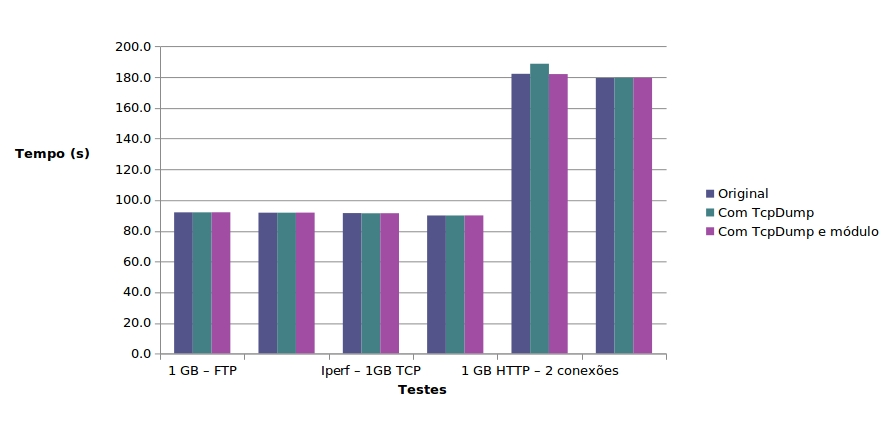
\includegraphics[scale=0.6]{testes.jpg}
\caption{Testes de desempenho efectuados ao MRoP}
\label{fig:tests_graphics}
\end{figure}

\begin{figure}[!ht]
\centering
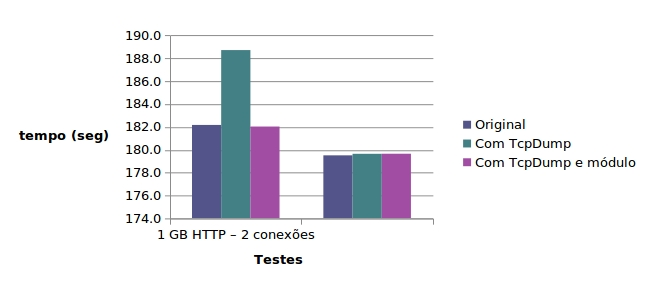
\includegraphics[scale=0.7]{overhead.jpg}
\caption{Sobrecarga nos testes 5 e 6 }
\label{fig:tests_overhead}
\end{figure}

Os primeiros 4 testes foram efectuados utilizando apenas uma conexão ao servidor, enquanto o 5º e o 6º testes utilizaram mais uma comunicação, de modo a aumentar o peso sobre o processador e o número de pacotes a circular entre as máquinas.
Desta forma, foi possível identificar a sobrecarga exercida enquando o \textit{tcpdump} executava e capturava todos os pacotes ou apenas um subconjunto destes, ou seja, os pacotes relativos aos processos alvo no novo sistema.
A coluna "Original" corresponde aos valores resultantes dos tempos médios das execuções das transferências na ausência de monitorização.
A coluna "Com \textit{TcpDump}" apresenta a média dos tempos de transferência com a captura total do tráfego utilizando a \textit{LibPCap}/\textit{LSF} original, enquanto que a coluna identificada com "Com \textit{TcpDump} e \textit{MRoP}" regista a média dos tempos para a transferência com captura pelo tcpdump e o módulo \textit{MRoP} desenvolvido no núcleo, de forma a capturar, apenas, o tráfego da transferência do processo alvo.
Nos primeiros quatro testes é possível verificar que a utilização do \textit{MRoP}, aumentou de forma insignificativa o tempo de execução (figura \ref{fig:tests_graphics}).
É igualmente possível observar que no 1º e 3º testes, aquando da utilização do \textit{tcpdump}, a execução sem o \textit{MRoP}, mostrou-se muito ligeiramente mais rápida, como se pode verificar na tabela \ref{tab:desempenho} e \ref{tab:overhead}.


Esta situação pode dever-se ao facto de, quando a máquina se encontra em sobrecarga, leva ao aumento do tamanho médio dos pacotes, reduzindo o seu número e o volume de dados transferidos, em virtude da diminuição dos seus cabeçalhos.

Nos testes 5º e 6º testes, como o tráfego na interface é duplicado e o \textit{tcpdump} tem que capturar todos os pacotes, é possível evidenciar a sobrecarga exercida por estas cópias de dados e consequentes transferências (para nível utilizador) face ao novo sistema onde apenas captura um fluxo de dados.
Na tabela \ref{tab:overhead} e na figura \ref{fig:tests_overhead} é possível observar que, para o teste 5, a sobrecarga do \textit{tcpdump} atinge os 3.6\% face ao original, enquanto que a sobrecarga do \textit{tcpdump} com o \textit{MRoP}, permitiu uma ligeira melhoria face ao original (-0.0775\%).
Conclui-se, portanto, que quando o fluxo de dados que não pretendemos capturar aumenta consideravelmente, torna-se mais vantajoso utilizar o \textit{MRoP}, do que capturar todos os pacotes, na medida em que minimiza-se a sobrecarga, capturando apenas os dados relevantes, evitando-se eventuais análise em nível utilizador, ou seja, na identificação e filtragem dos pacotes pertencentes ao processo alvo (o que acarretaria uma sobrecarga adicional).

\subsection{Desempenho da estrutura de dados}

Para além das avaliações anteriormente descritas, tornou-se essencial analisar o comportamento da estrutura de dados utilizado no componente “estado do processo”, de modo a verificar o seu desempenho.
Assim para esta análise, foi elaborado um teste que utiliza o sistema de alta resolução de temporizadores (\textit{HRTimer})\cite{hrtimerKernel}, contido no núcleo do sistema de operação.

O teste consistiu em obter o tempo anterior e posterior à inserção dos 1024 elementos, representando outros tantos portos/endereços, afim de determinar o tempo decorrido.
De igual modo, foi calculado o tempo de remoção dos referidos elementos. Os resultados obtidos estão reproduzidos na tabela \ref{tab:tree_info}.

\begin{table}[!htb]
\begin{center}
\caption{Custo das operações (tempos em nanosegundos)}
\begin{tabular}{ | r | c | c | }
\hline
\hspace{1cm} Teste \hspace{1.5cm} & \hspace{1cm}Duração\hspace{1cm} &  Média por
elemento \\
\hline
Adição de 1024 elementos & 869 244 & 848.8711 \\
\hline
Remoção de 1024 elementos & 675 086 & 659.2637\\
\hline

\hline
\end{tabular}
\label{tab:tree_info}
\end{center}
\end{table}

Como se pode verificar, pela tabela \ref{tab:tree_info}, a inserção de um elemento na árvore é inferior a 1 microsegundo, possivelmente demonstrando que a estrutura utilizada foi a correcta.
Para além de estabelecer um bom compromisso de desempenho e utilização de memória, a sua disponibilidade de utilização no núcleo do sistema, possibilitou obter ter um elevado grau de confiança na sua utilização.
O tempo médio despendido na procura do elemento com o menor valor de chave, nos 1024 elementos adicionados, foi de 1327 nanosegundos.
Com este valor é possível verificar que para efectuar 10 iterações de procura na árvore, incorre-se numa penalização de 1.3 microsegundos.
Verifica-se assim, que o tempo médio de procura de elementos na estrutura, é menor ou igual a 1.3 microsegundos.
Considerando que a maioria das aplicações não utiliza tantos portos em simultâneo, são expectáveis tempos inferiores em aplicações reais.


\subsection{Desempenho do Sistema de instrumentação}
Sendo a instrumentação das chamadas ao sistema um ponto fundamental na execução da monitorização de uma aplicação, a análise ao seu comportamento é bastante importante, na medida em que é necessário verificar se a introdução deste tipo de sistema irá produzir uma elevada penalização sobre o sistema de operação.
A análise efectuada consistiu em colocar um \textit{KRetProbe} na chamada ao sistema \textit{getpid} e avaliar o tempo decorrido entre o início e o fim do total das chamadas, com e sem o \textit{KRetProbe}, de forma a avaliar a sobrecarga e verificar se coincide com o indicado pelos criadores do sistema.
A chamada ao sistema escolhida foi o \textit{getpid}, pois esta é uma função muito simples que apenas devolve o identificador do processo que a invocou.

\providecommand{\e}[1]{\ensuremath{\times 10^{#1}}}

\begin{table}[!htb]
\begin{center}
\caption{Duração das chamadas em segundos}
\begin{tabular}{ | c | c | c | c |}
\hline
Teste & Original & Com \textit{KRetProbe} & Sobrecarga por chamada\\
\hline
100 000 000 chamadas & 12.65 &  73.6600 & 610.10\e{-9}\\
1 000 000 000 chamadas & 126.85 & 737.2100 & 610.36\e{-9}\\
\hline
\end{tabular}
\label{tab:kprobes_info}
\end{center}
\end{table}

Os valores de referência nos manuais do \textit{KRetProbe} são de 0.7 microsegundos\cite{KProbeKernel}, sendo que os valores obtidos foram de 0.61 microsegundos, ou seja, ligeiramente inferiores, visto que a máquina de referência apresenta frequências de \textit{cpu} inferiores à máquina onde foram realizados estes testes.

Consideram-se estes valores bastante aceitáveis e espera-se que tenham ainda pouco impacto no desempenho normal do sistema.
Note-se ainda que esta instrumentação só é introduzida aquando do carregamento do módulo para executar a monitorização com esta nova funcionalidade.

\section{Conclusão}


